%% liftarm.tex
%% Copyright 2022-2024 Matthias Floré
%
% This work may be distributed and/or modified under the
% conditions of the LaTeX Project Public License, either version 1.3c
% of this license or (at your option) any later version.
% The latest version of this license is in
%   http://www.latex-project.org/lppl.txt
% and version 1.3c or later is part of all distributions of LaTeX
% version 2005/12/01 or later.
%
% This work has the LPPL maintenance status `maintained'.
% 
% The Current Maintainer of this work is Matthias Floré.
%
% This work consists of the files liftarm.pdf, liftarm.sty,
% liftarm.tex and README.md.
\documentclass[a4paper,english,dvipsnames]{ltxdoc}
\usepackage[english]{babel}
\usepackage{graphicx}
\usepackage[a4paper,left=2.25cm,right=2.25cm,top=2.5cm,bottom=2.5cm,nohead]{geometry}
\usepackage{parskip}
\usepackage{iftex}
\ifluatex
\else
\usepackage[T1]{fontenc}
\usepackage[utf8]{inputenc}
\fi
\usepackage{mathtools}
\usepackage{amssymb}
\allowdisplaybreaks
\usepackage{pdflscape}
\usepackage{animate}
\usepackage{liftarm}
\input{pgfmanual-en-macros.tex}
\usepackage{codehigh}
\usepackage{fancyhdr}
\pagestyle{fancy}
\renewcommand{\headrulewidth}{0pt}
\fancyhead{}
\fancyfoot[C]{\IfRefUndefinedExpandable{Thesourcecode}{}{\begin{tikzpicture}\liftarm[mark holes=\thepage -1]{0,0}{\getpagerefnumber{Thesourcecode}-2}{0}\end{tikzpicture}}}%\liftarm{0,0}{\thepage}{0}
\usepackage[nottoc]{tocbibind}
\usepackage{imakeidx}
\makeindex[program=makeindex,columns=2,intoc=true]
\indexsetup{othercode={\thispagestyle{fancy}}}
\usepackage[linktoc=all,pdfstartview=FitH,colorlinks=true,linkcolor=Mahogany,citecolor=ForestGreen,urlcolor=MidnightBlue,bookmarksnumbered=true]{hyperref}
\hypersetup{pdftitle={The liftarm package},pdfauthor={Matthias Floré},pdfsubject={Manual},pdfkeywords={liftarm}}
\setcounter{tocdepth}{2}
\setcounter{secnumdepth}{2}
\DeclareMathOperator{\atan}{atan}
\title{The \texttt{liftarm} package\\[12pt]\large Geometric constructions with liftarms using \tikzname{} and \LaTeX3}
\author{Matthias Floré}
\date{Version 3.0 (2024/05/20)}%\\[12pt]
\begin{document}
\maketitle
\thispagestyle{fancy}
\begin{abstract}
\noindent This package is based on the package |tikz| (see \cite{TtTaPGFp}) and can be used to draw geometric constructions with liftarms using \tikzname. There are several options for the appearance of the liftarms. It provides an environment to connect multiple liftarms using the Newton-Raphson method and LU decomposition. It also provides an environment to describe a construction and a method to animate a construction with one or more traces.% This is the manual for version .
\end{abstract}
\tableofcontents
\section{Usage}
The package |liftarm| can be used by putting the following in the preamble.
\begin{codeexample}[code only]
\usepackage{liftarm}
\end{codeexample}
The package |liftarm| loads the package |xcolor| with the option |dvipsnames|, the package |tikz| and the \tikzname{} library |calc|. Since |xcolor| is loaded with the option |dvipsnames|, packages such as |pgfplots| and |tcolorbox| must be loaded \emph{after} |liftarm|.
\section{Drawing liftarms}
\begin{command}{\liftarm\opt{\oarg{options}}\marg{point}\marg{length}\marg{angle}}
This command can be placed inside a |tikzpicture| environment. It draws a liftarm of \meta{length} starting at \meta{point}. The angle between the liftarm and the $x$-axis can be specified by \meta{angle} in degrees. The distance between the holes is $1$.
\begin{codeexample}[width=10cm]
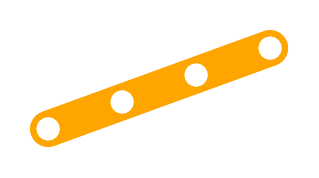
\begin{tikzpicture}
\liftarm{1,2}{3}{20}
\end{tikzpicture}
\end{codeexample}
Note that the number of holes is $\meta{length}+1$. The \meta{options} can be given with the following keys.
\begin{key}{/liftarm/axle holes=\marg{values}}
This key defines the holes in the liftarm where axle holes will be drawn.
\begin{codeexample}[width=10cm]

\begin{tikzpicture}
\liftarm[axle holes={0,4}]{0,1}{4}{0}
\end{tikzpicture}
\end{codeexample}
\end{key}
\begin{key}{/liftarm/brick=\opt{\meta{boolean}} (default true, initially false)}
If true, a brick will be drawn instead of a liftarm.
\begin{codeexample}[width=10cm]

\begin{tikzpicture}
\liftarm[brick]{0,1}{2}{0}
\end{tikzpicture}
\end{codeexample}
\end{key}
\begin{key}{/liftarm/color=\marg{number}\marg{color}}
This key defines the color of liftarms of length \meta{number}.

Initially, the colors |Gray|, |darkgray|, |Yellow|, |Orange|, |Red|, |Green|, |Blue| and |Brown| are defined for respectively the lengths |0| till |7|.
\end{key}
\begin{key}{/liftarm/color modulo=\marg{number} (initially 8)}
The default colors of the liftarms are determined by computing the length of the liftarm modulo the value of this key and selecting the color defined by the key |color|.
\begin{codeexample}[width=10cm]
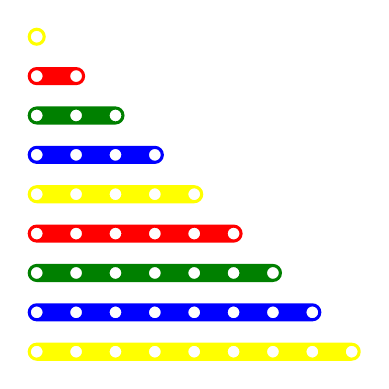
\begin{tikzpicture}[scale=0.5]
\pgfkeys{
  /liftarm,
  color={0}{Yellow},
  color={1}{Red},
  color={2}{Green},
  color={3}{Blue},
  color modulo=4
}
\foreach\n in {0,...,8}{
  \liftarm{0,-\n}{\n}{0}
}
\end{tikzpicture}
\end{codeexample}
\end{key}
\begin{key}{/liftarm/contour=\opt{\meta{boolean}} (default true, initially false)}
If true, a contour will be drawn around the liftarm.
\begin{codeexample}[width=10cm]
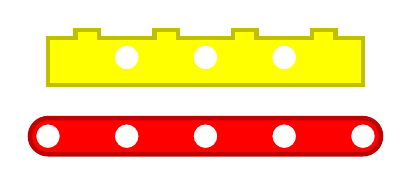
\begin{tikzpicture}
\liftarm[contour]{0,1}{4}{0}
\liftarm[brick,contour]{1,2}{2}{0}
\end{tikzpicture}
\end{codeexample}
\end{key}
\begin{stylekey}{/liftarm/contour style=\marg{options} (initially \normalfont empty)}
The style of the contour is determined as follows. First, the color is defined as \meta{initial color of the liftarm}|!75!black|. Then the option |ultra thick| is added. Thereafter, the style of the key |contour style| is added.

The style |contour style| only applies to the border of the liftarm. The style |liftarm style| also applies to the holes of the liftarm.
\begin{codeexample}[width=10cm]
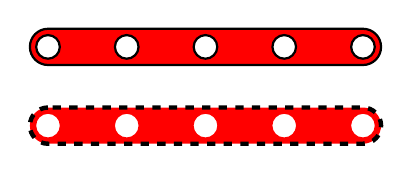
\begin{tikzpicture}
\liftarm[
  contour,
  contour style={dashed,black}
]{0,1}{4}{0}
\liftarm[
  liftarm style={draw=black,thick}
]{0,2}{4}{0}
\end{tikzpicture}
\end{codeexample}
\end{stylekey}
\begin{key}{/liftarm/coordinate=\marg{number 1/name 1,\dots}}
This key defines coordinates with name \meta{name i} at hole \meta{number i} of the liftarm.
\begin{codeexample}[width=10cm]
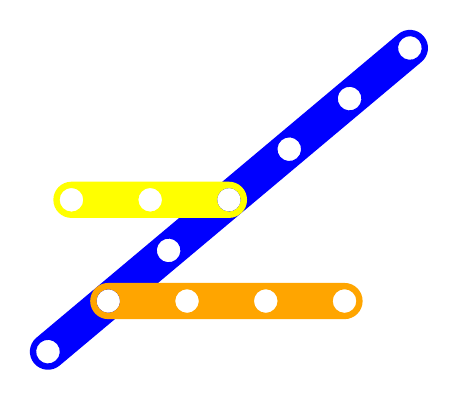
\begin{tikzpicture}
\liftarm[
  coordinate={1/A,3/B}
]{0,1}{6}{40}
\liftarm{A}{3}{0}
\liftarm{B}{2}{180}
\end{tikzpicture}
\end{codeexample}
\end{key}
\begin{key}{/liftarm/hole radius=\marg{value} (initially 0.3)}
The \meta{value} of this key, multiplied with the \meta{value} of the key |scalefactor| defines the radius of the holes.
\begin{codeexample}[width=10cm]

\begin{tikzpicture}
\liftarm[hole radius=0.1]{0,0}{5}{0}
\end{tikzpicture}
\end{codeexample}
\end{key}
\begin{stylekey}{/liftarm/liftarm style=\marg{options} (initially \normalfont empty)}
The style of the liftarm is determined as follows. First, the color is defined by the keys |color| and |color modulo|. Thereafter, the style of the key |liftarm style| is added.
\end{stylekey}
\begin{key}{/liftarm/liftarm thickness=\marg{value} (initially 0.92)}
The \meta{value} of this key, multiplied with the \meta{value} of the key |scalefactor| defines the thickness of the liftarm.
\begin{codeexample}[width=10cm]

\begin{tikzpicture}
\liftarm[
  hole radius=0.1,
  liftarm thickness=0.3
]{0,0}{5}{0}
\end{tikzpicture}
\end{codeexample}
\end{key}
\begin{key}{/liftarm/mark holes=\marg{values}}
\end{key}
\begin{key}{/liftarm/mark radius=\marg{factor} (initially 1)}
\end{key}
\begin{stylekey}{/liftarm/mark style=\marg{options} (initially \normalfont empty)}
The key |mark holes| defines the holes in the liftarm which will be marked. The radius is the product of the \meta{factor} given to the key |mark radius| and the value of the key |hole radius|. The style of these marks is determined as follows. First, the color is set to |black|. Thereafter, the style of the key |mark style| is added.
\begin{codeexample}[width=10cm]
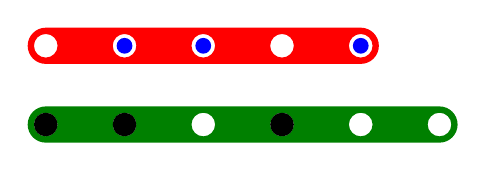
\begin{tikzpicture}
\liftarm[
  mark holes={0,1,3}
]{0,0}{5}{0}
\liftarm[
  mark holes={1,2,4},
  mark radius=2/3,
  mark style=Blue
]{0,1}{4}{0}
\end{tikzpicture}
\end{codeexample}
\end{stylekey}
\begin{key}{/liftarm/origin=\marg{number} (initially 0)}
This key defines the number of the hole which will be placed at the coordinate given as argument to the liftarm.
\begin{codeexample}[width=10cm]
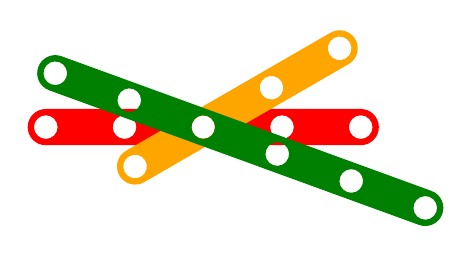
\begin{tikzpicture}
\liftarm{-2,0}{4}{0}
\liftarm[origin=1]{0,0}{3}{30}
\liftarm[origin=2]{0,0}{5}{-20}
\end{tikzpicture}
\end{codeexample}
\end{key}
\begin{key}{/liftarm/scalefactor=\marg{value} (initially 0.5)}
The \meta{value} of this key defines the factor which scales the thickness of the liftarm and the radius of the holes.
\begin{codeexample}[width=10cm]
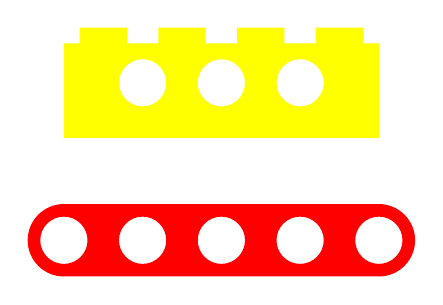
\begin{tikzpicture}
\liftarm[scalefactor=1]{0,0}{4}{0}
\liftarm[brick,scalefactor=1]{1,2}{2}{0}
\end{tikzpicture}
\end{codeexample}
\end{key}
\begin{key}{/liftarm/screw angle=\marg{angle} (initially 10)}
\end{key}
\begin{key}{/liftarm/screw holes=\marg{values}}
\end{key}
\begin{key}{/liftarm/screw radius=\marg{factor} (initially 0.8)}
\end{key}
\begin{stylekey}{/liftarm/screw style=\marg{options} (initially \normalfont empty)}
The key |screw holes| defines the holes in the liftarm where a screw will be drawn. The angle of these screws is determined by the key |screw angle| which is an angle in degrees. The radius is the product of the \meta{factor} given to the key |screw radius| and the value of the key |hole radius|. The style of these screws is determined as follows. First, the color is set to |black|. Then the option |rotate=45| is added. Thereafter, the style of the key |screw style| is added.
\begin{codeexample}[width=10cm]
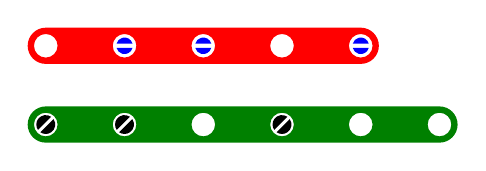
\begin{tikzpicture}
\liftarm[
  screw holes={0,1,3}
]{0,0}{5}{0}
\liftarm[
  screw angle=15,
  screw holes={1,2,4},
  screw radius=0.7,
  screw style={Blue,rotate=-45}
]{0,1}{4}{0}
\end{tikzpicture}
\end{codeexample}
\end{stylekey}
\begin{key}{/liftarm/type=\mchoice{liftarm,line segment} (initially liftarm)}
\begin{description}
\item[\texttt{liftarm}] In this case, the command |\liftarm| draws a liftarm.
\item[\texttt{line segment}] In this case, the command |\liftarm| draws a line segment.
\end{description}
\end{key}
\end{command}
\section{Connecting liftarms}
\begin{environment}{{liftarmconnect}\opt{\oarg{options}}}
This environment can be placed inside a |tikzpicture| environment. It can be used to connect liftarms where the angles are computed automatically. The \meta{options} can be a list of keys from the liftarm key family.

The contents should consist only of commands |\liftarm| and spaces.

The conditions to connect the liftarms are specified by the key |coordinate|. The resulting equations are determined automatically by the environment |liftarmconnect|. The number of liftarms needs to be equal to the number of equations. In the example below, there are 2 liftarms and 1 condition specified with the coordinate |A| resulting in 2 equations.
\begin{codeexample}[width=10cm]
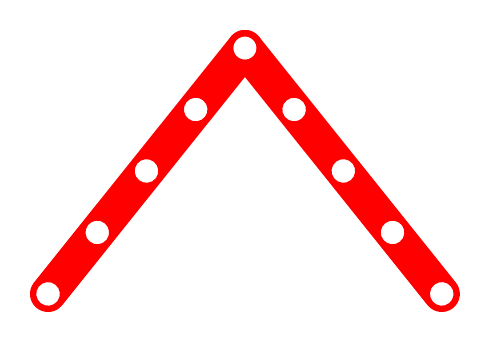
\begin{tikzpicture}
\coordinate (X) at (5,0);
\begin{liftarmconnect}
  \liftarm[coordinate=4/A]{0,0}{4}{60}
  \liftarm[coordinate=4/A]{X}{4}{120}
\end{liftarmconnect}
\end{tikzpicture}
\end{codeexample}
The similar code below does not work because the coordinate |A| is used as the starting point of the second liftarm but is unknown since it is used in a condition for the first liftarm and furthermore, there is no liftarm to complement the condition involving |A| in the first liftarm.
\begin{codeexample}[code only]
\begin{tikzpicture}
\coordinate (X) at (5,0);
\begin{liftarmconnect}
  \liftarm[coordinate=4/A]{0,0}{4}{60}
  \liftarm[coordinate=4/X]{A}{4}{-60}
\end{liftarmconnect}
\end{tikzpicture}
\end{codeexample}
If the environment |liftarmconnect| consists of 2 liftarms then the law of cosines is used to compute the angles.

If there are more than 2 liftarms then the set of equations is solved with the Newton-Raphson method. The initial values for the angles are given by the last arguments of the commands |\liftarm|. The Jacobian matrix is defined by the environment |liftarmconnect|. The resulting set of linear equations is solved with LU decomposition. The iteration stops if the condition determined by the key |connect stop| is satisfied.

Since the \emph{let operation} from the \tikzname{} library |calc| is used, it is not possible to use the variable names |\n|, |\p|, |\x| and |\y| inside the starting point of a command |\liftarm| which is used in the environment |liftarmconnect|.
\begin{key}{/liftarm/connect stop=\mchoice{1-norm,2-norm,iterations} (initially 1-norm)}
\begin{description}
\item[\texttt{1-norm}] In this case, the iteration stops if the 1-norm is smaller than the value given to this key. Its default value is $0.001$.
\item[\texttt{2-norm}] In this case, the iteration stops if the 2-norm is smaller than the value given to this key. Its default value is $0.001$.
\item[\texttt{iterations}] In this case, a number of iterations is executed where the number is the one given to this key. Its default value is $10$.
\end{description}
\end{key}
\begin{codeexample}[width=10cm]
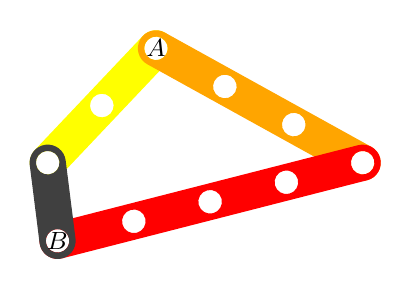
\begin{tikzpicture}
\begin{liftarmconnect}
  \liftarm[coordinate=2/A]{0,0}{2}{70}
  \liftarm[coordinate=3/A]{4,0}{3}{120}
\end{liftarmconnect}
\begin{liftarmconnect}
  \liftarm[coordinate=4/B]{4,0}{4}{200}
  \liftarm[coordinate=1/B]{0,0}{1}{-90}
\end{liftarmconnect}
\node at (A) {\small $A$};
\node at (B) {\small $B$};
\end{tikzpicture}
\end{codeexample}
The example below shows the regular pentagon from \cite{Tmm1}. In the first environment |liftarmconnect| there are $4$ liftarms and $2$ conditions resulting in $4$ equations. Hence the Jacobian matrix has size $4\times 4$.
\begin{codeexample}[width=7cm]
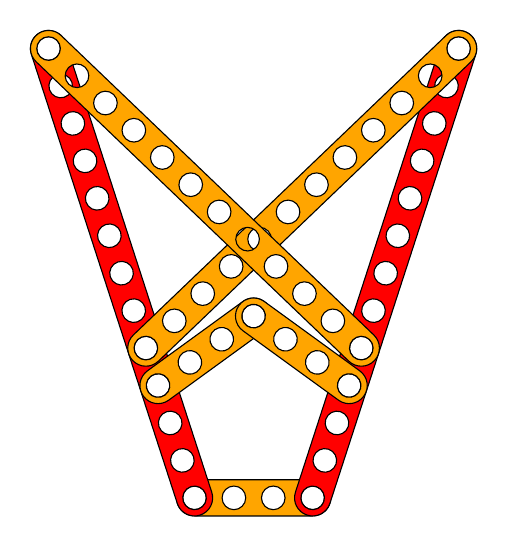
\begin{tikzpicture}[scale=0.5]
\pgfkeys{/liftarm,liftarm style={draw=black},scalefactor=1}
\liftarm{0,0}{3}{0}
\begin{liftarmconnect}
  \liftarm[coordinate={3/A,4/B,12/C}]{0,0}{12}{100}
  \liftarm[coordinate={3/D,4/E,12/F}]{3,0}{12}{80}
  \liftarm[coordinate=11/F]{B}{11}{60}
  \liftarm[coordinate=11/C]{E}{11}{120}
\end{liftarmconnect}
\begin{liftarmconnect}
  \liftarm[coordinate=3/G]{A}{3}{30}
  \liftarm[coordinate=3/G]{D}{3}{150}
\end{liftarmconnect}
\end{tikzpicture}
\end{codeexample}
The example below shows iterations $0$ till $3$ of a construction with $6$ liftarms and $3$ conditions resulting in $6$ equations. Hence the Jacobian matrix has size $6\times 6$.
\begin{codeexample}[]
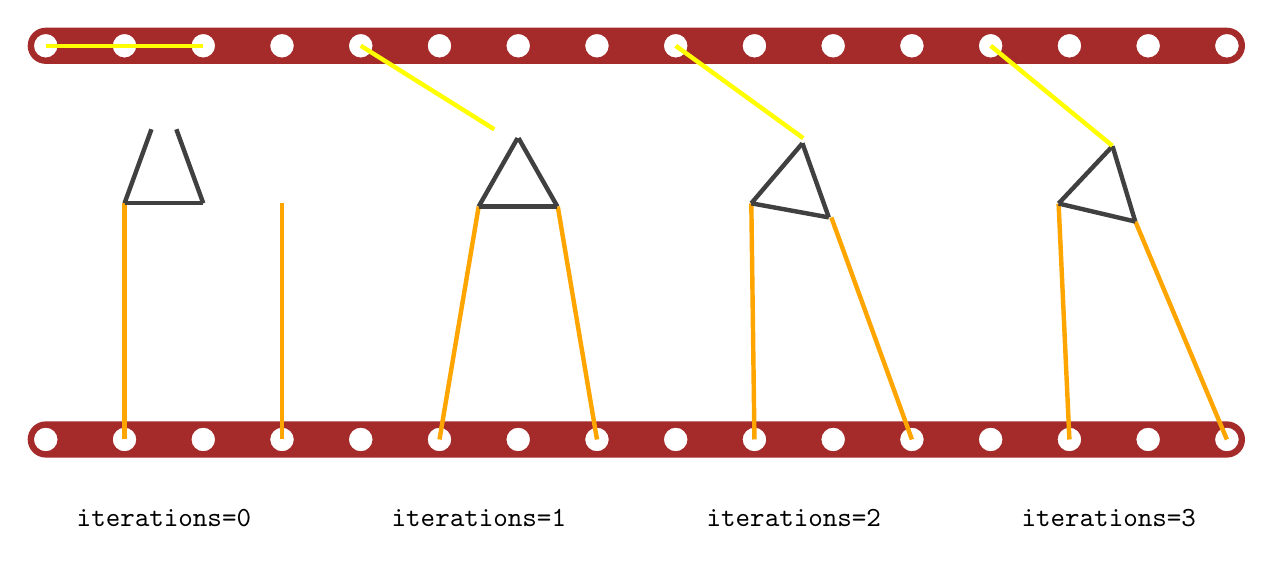
\begin{tikzpicture}
\liftarm{0,0}{15}{0}
\liftarm{0,5}{15}{0}
\foreach\k in {0,...,3}{
  \begin{scope}[shift={(\k*4,0)}]
    \begin{liftarmconnect}[connect stop={iterations=\k},liftarm style=ultra thick,type=line segment]
      \liftarm[coordinate=3/A]{1,0}{3}{90}
      \liftarm[coordinate=3/B]{3,0}{3}{90}
      \liftarm[coordinate=1/B]{A}{1}{0}
      \liftarm[coordinate=1/C]{A}{1}{70}
      \liftarm[coordinate=1/C]{B}{1}{110}
      \liftarm[coordinate=2/C]{0,5}{2}{0}
    \end{liftarmconnect}
    \node at (1.5,-1) {\texttt{iterations=\k}};
  \end{scope}
}
\end{tikzpicture}
\end{codeexample}
The example below shows the regular heptagon from \cite{Tmm1}. In the first environment |liftarmconnect| there are $8$ liftarms and $4$ conditions resulting in $8$ equations. Hence the Jacobian matrix has size $8\times 8$.
\begin{codeexample}[width=8cm]

\begin{tikzpicture}[scale=0.4]
\pgfkeys{/liftarm,scalefactor=1}
\liftarm{-4,0}{8}{0}
\begin{liftarmconnect}
  \liftarm[coordinate={1/A,7/B,8/G}]{-4,0}{8}{135}
  \liftarm[coordinate=11/F]{A}{11}{50}
  \liftarm[coordinate=11/F]{B}{11}{20}
  \liftarm[coordinate={1/C,7/D,8/H}]{4,0}{8}{45}
  \liftarm[coordinate=11/E]{C}{11}{130}
  \liftarm[coordinate=11/E]{D}{11}{160}
  \liftarm[coordinate=8/E]{G}{8}{30}
  \liftarm[coordinate=8/F]{H}{8}{150}
\end{liftarmconnect}
\begin{liftarmconnect}
  \liftarm[coordinate=8/I]{E}{8}{70}
  \liftarm[coordinate=8/I]{F}{8}{110}
\end{liftarmconnect}
\begin{liftarmconnect}
  \liftarm[coordinate=8/J]{G}{8}{70}
  \liftarm[coordinate=8/J]{I}{8}{210}
\end{liftarmconnect}
\begin{liftarmconnect}
  \liftarm[coordinate=8/K]{H}{8}{110}
  \liftarm[coordinate=8/K]{I}{8}{-30}
\end{liftarmconnect}
\end{tikzpicture}
\end{codeexample}
\end{environment}
\section{Describing a construction}
If a construction involves many liftarms then it is convenient to describe this construction in separate steps. Then the content of previous steps would need to be copied in each new step. This process can be automated by using the command |\liftarmconstruct| below.
\begin{command}{\liftarmconstruct\marg{commands}}
This command appends \meta{commands} to an internal token list. Then it uses this token list.
\end{command}
\begin{command}{\liftarmconstructclear}
This command clears the token list which is used by the command |\liftarmconstruct|.

As an example, we describe below the construction of a regular pentagon from \cite{Tmm1}.
\begin{codeexample}[width=7cm]
\begin{minipage}{5.5cm}%only for usage in this manual
\liftarmconstructclear
\begin{enumerate}
\item First we form a rectangular triangle with 3 liftarms.
\begin{center}
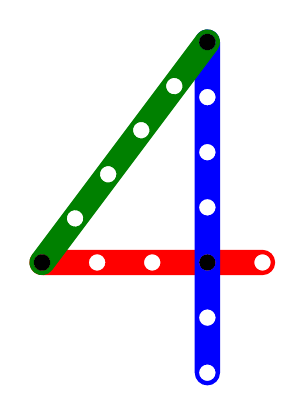
\begin{tikzpicture}[scale=0.7]
\liftarmconstruct{
  \liftarm[mark holes=3]{-3,0}{4}{0}
  \begin{liftarmconnect}
    \liftarm[coordinate=6/A,origin=2]{0,0}{6}{90}
    \liftarm[coordinate=5/A,mark holes={0,5}]{-3,0}{5}{60}
  \end{liftarmconnect}
}
\end{tikzpicture}
\end{center}
\item Then we add 2 liftarms of length $3$.
\begin{center}
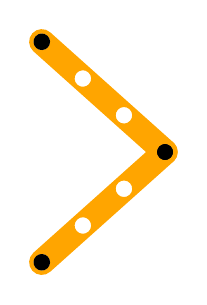
\begin{tikzpicture}[scale=0.7]
\liftarmconstruct{
  \begin{liftarmconnect}
    \liftarm[coordinate=3/B,mark holes={0,3}]{0,-2}{3}{45}
    \liftarm[coordinate=3/B,mark holes=0]{0,2}{3}{-45}
  \end{liftarmconnect}
}
\end{tikzpicture}
\end{center}
\item Here appears the first side of the regular pentagon.
\begin{center}
\begin{tikzpicture}[scale=0.7]
\liftarmconstruct{
  \begin{liftarmconnect}
    \liftarm[coordinate=2/C]{B}{2}{100}
    \liftarm[coordinate=2/C,mark holes={0,2}]{1,0}{2}{80}
  \end{liftarmconnect}
}
\end{tikzpicture}
\end{center}
\item Now we end the construction of the regular pentagon.
\begin{center}
\begin{tikzpicture}[scale=0.7]
\liftarmconstruct{
  \begin{liftarmconnect}
    \liftarm[coordinate=2/D]{C}{2}{180}
    \liftarm[coordinate=2/D,mark holes={0,2}]{-1,0}{2}{80}
  \end{liftarmconnect}
  \begin{liftarmconnect}
    \liftarm[coordinate=2/E,mark holes=2]{-1,0}{2}{-80}
    \liftarm[coordinate=2/E]{B}{2}{210}
  \end{liftarmconnect}
}
\end{tikzpicture}
\end{center}
\end{enumerate}
\end{minipage}
\end{codeexample}
\end{command}
\section{Animations}
\begin{command}{\liftarmanimate\opt{\oarg{options}}\marg{frame rate}\marg{list}\marg{command}}
This command shows an animation using the |animateinline| environment of the package |animate|. The package |animate| is \emph{not} loaded by default and needs to be loaded to use the command |\liftarmanimate|. The \meta{options} are passed to the |animateinline| environment. The \meta{frame rate} of the animation is described in the documentation of the package |animate|. The \meta{command} must be a previously defined command with one mandatory argument. The \meta{list} is passed to a |\foreach| loop. The frames of the animation consist of the \meta{command} evaluated one by one in the result of the |\foreach| loop. The command |\liftarmanimate| creates a timeline which is used in the |animateinline| environment. This timeline is stored in the file \meta{job name}\meta{number of the animation in the document}|.tln|. It requires two compiler runs to create and use this timeline correctly.
\begin{key}{/liftarm/trace=\marg{number/number of frames/code}\dots}
This key draws \meta{code} at hole \meta{number} of the liftarm on the frames of the animation determined by \meta{number of frames}.

If \meta{number of frames} is 0 then the \meta{code} is drawn starting at the current frame until the end of the animation. If \meta{number of frames} is an integer greater than or equal to 1 then the \meta{code} is drawn starting at the current frame and remaining during the next frames determined by \meta{number of frames}. If \meta{number of frames} is left empty then the \meta{code} is drawn starting at the beginning of the animation until the end of the animation.

The \meta{code} can be some \tikzname{} code. In this \meta{code}, $(0,0)$ is positioned at hole \meta{number} of the liftarm. If \meta{code} is left empty then a black circle with radius $\frac{2}{3}$ times the |hole radius| is used.

A list of multiple triples \meta{number/number of frames/code} can be given to the key |trace|.
\begin{codeexample}[width=10cm,preamble={\usepackage{animate}}]
\newcommand{\exampleliftarmanimate}[1]{
  \liftarm[
    origin=1,
    mark holes=1,
    trace={
      2/0/,
      3//,
      4/3/{\fill[Blue] (0,0)
        circle[radius=0.15];}
    }
  ]{0,0}{4}{#1}
}
\liftarmanimate[
  autoplay,
  controls,
  loop,
  begin={
    \begin{tikzpicture}
    \useasboundingbox (-4,-4)
      rectangle (4,4);
  },
  end={\end{tikzpicture}}
]
{5}
{0,30,...,330}
{\exampleliftarmanimate}
\end{codeexample}
\end{key}
\end{command}
\section{Additional examples}
The following example shows a regular hexagon.
\begin{codeexample}[width=8cm]

\begin{tikzpicture}
\def\r{3}
\foreach\m in {1,...,6}{
  \begin{liftarmconnect}
    \liftarm[coordinate=\r/A]{0,0}{\r}{(\m+1)*60}
    \liftarm[coordinate=\r/A]{\m*60:\r}{\r}{(\m+2)*60}
  \end{liftarmconnect}
}
\end{tikzpicture}
\end{codeexample}
The following example illustrates that $2\atan(\frac{1}{2})=\atan(\frac{4}{3})$.
\begin{codeexample}[width=9cm]
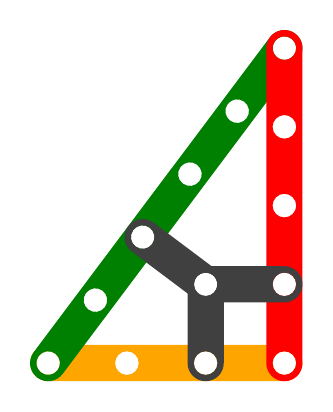
\begin{tikzpicture}
\liftarm{0,0}{3}{0}
\liftarm{0,0}{5}{atan(4/3)}
\liftarm{3,0}{4}{90}
\liftarm{2,0}{1}{90}
\liftarm{2,1}{1}{0}
\liftarm{2,1}{1}{90+atan(4/3)}
\end{tikzpicture}
\end{codeexample}
The following example illustrates an angle bisection.
\begin{codeexample}[width=9cm]
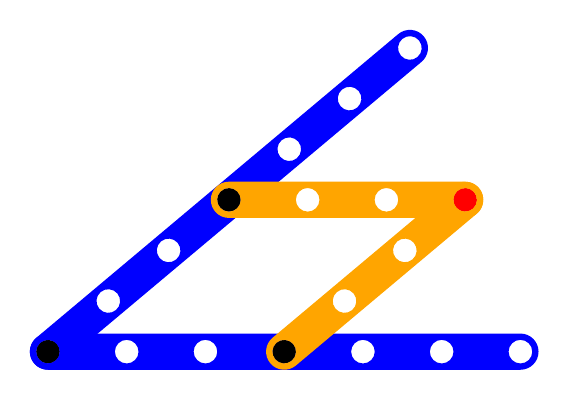
\begin{tikzpicture}
\def\ang{40}
\def\r{3}
\liftarm[mark holes={0,\r}]{0,0}{2*\r}{0}
\liftarm[mark holes=\r]{0,0}{2*\r}{\ang}
\liftarm[
  mark holes=\r,
  mark style=Red
]{\r,0}{\r}{\ang}
\liftarm{\ang:\r}{\r}{0}
\end{tikzpicture}
\end{codeexample}
The following example illustrates that $7^{2}=3^{2}+8^{2}-2\cdot 3\cdot 8\cos(\frac{\pi}{3})$.
\begin{codeexample}[width=9cm]
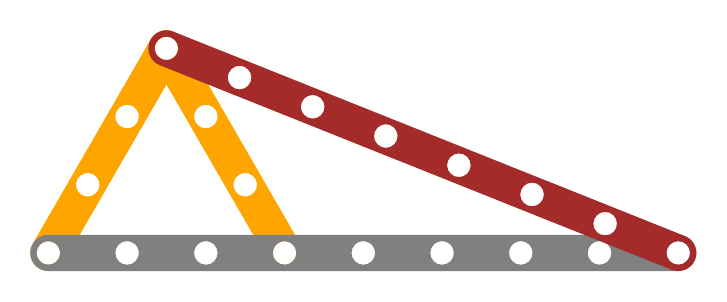
\begin{tikzpicture}
\begin{liftarmconnect}
  \liftarm[coordinate=3/A]{0,0}{3}{80}
  \liftarm[coordinate=3/A]{3,0}{3}{100}
\end{liftarmconnect}
\begin{liftarmconnect}
  \liftarm[coordinate=8/B]{0,0}{8}{0}
  \liftarm[coordinate=7/B]{A}{7}{0}
\end{liftarmconnect}
\end{tikzpicture}
\end{codeexample}
The following example illustrates that $7^{2}+4^{2}=8^{2}+1^{2}$.
\begin{codeexample}[width=9cm]
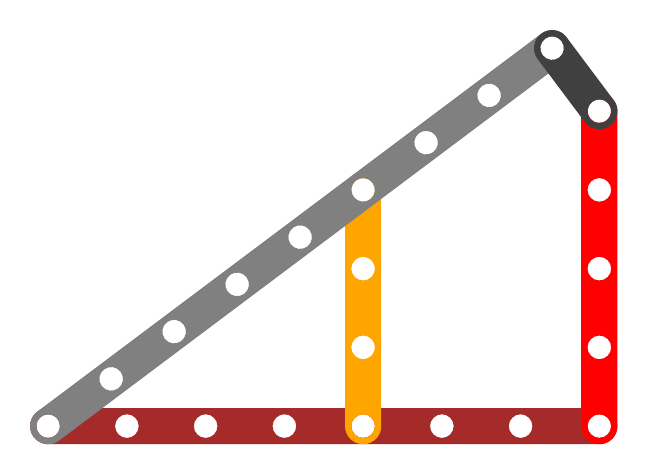
\begin{tikzpicture}
\def\a{4}
\def\b{7}
\def\c{1}
\def\d{8}
%\liftarm{0,0}{\b}{0}
%\liftarm{\b,0}{\a}{90}
\begin{liftarmconnect}
  \liftarm[coordinate=\b/A]{0,0}{\b}{0}
  \liftarm[coordinate=\a/A]{\b,\a}{\a}{-90}
\end{liftarmconnect}
\liftarm{4,0}{3}{90}
%\liftarm{\b,\a}{1}{atan(\a/\b)+atan(\c/\d)+90}
%\liftarm{0,0}{\d}{atan(\a/\b)+atan(\c/\d)}
\begin{liftarmconnect}
  \liftarm[coordinate=\d/B]{0,0}{\d}{45}
  \liftarm[coordinate=\c/B]{\b,\a}{\c}{135}
\end{liftarmconnect}
\end{tikzpicture}
\end{codeexample}
Below is an animation of the Peaucellier-Lipkin linkage, see e.g.~\cite{Koagmopermbl}.
\begin{codeexample}[width=9cm,preamble={\usepackage{animate}}]
\newcommand{\PLlinkage}[1]{
\begin{tikzpicture}[scale=0.75]
\def\a{3}
\def\b{4}
\def\c{9}
\edef\l{
  \fpeval{2*\a+(\c^2-\b^2-(2*\a)^2)/(2*\a)}
}
\useasboundingbox (-0.23,-6) rectangle
  (\l+0.23,6);
\draw (\l,-5)--(\l,5);
\liftarm{0,0}{\a}{0}
\liftarm[coordinate=\a/A]{\a,0}{\a}{#1}
\begin{liftarmconnect}
  \liftarm[coordinate=\c/B]{0,0}{\c}{0}
  \liftarm[coordinate=\b/B]{A}{\b}{90}
\end{liftarmconnect}
\begin{liftarmconnect}
  \liftarm[coordinate=\c/C]{0,0}{\c}{0}
  \liftarm[coordinate=\b/C]{A}{\b}{-90}
\end{liftarmconnect}
\begin{liftarmconnect}
  \liftarm[coordinate=\b/D]{C}{\b}{0}
  \liftarm[coordinate=\b/D]{B}{\b}{0}
\end{liftarmconnect}
\end{tikzpicture}
}
\begin{animateinline}[
  autoplay,
  controls,
  palindrome
]{30}
\multiframe{80}{rAng=-40+1}{
  \PLlinkage{\rAng}
}
\end{animateinline}
\end{codeexample}
Below is an animation of Kempe's trisector, as shown in \cite{Tmm3}.
\begin{codeexample}[preamble={\usepackage{animate}}]
\newcommand{\trisector}[1]{
\begin{tikzpicture}[scale=0.33]
\useasboundingbox (-27.3,-0.5) rectangle (21.2,37);
\liftarm[coordinate=8/A]{0,0}{27}{180}
\liftarm[coordinate=12/B]{0,0}{27}{180-(#1)}
\liftarm[coordinate=18/C]{0,0}{27}{180-2*(#1)}
\liftarm[coordinate=27/D]{0,0}{27}{180-3*(#1)}
\begin{liftarmconnect}
  \liftarm[coordinate=27/E]{C}{27}{0}
  \liftarm[coordinate=18/E]{D}{18}{0}
\end{liftarmconnect}
\begin{liftarmconnect}
  \liftarm[coordinate=12/F]{A}{12}{0}
  \liftarm[coordinate=8/F]{B}{18}{0}
\end{liftarmconnect}
\end{tikzpicture}
}
\begin{animateinline}[autoplay,controls,palindrome]{5}
\multiframe{20}{rAng=15+1}{
  \trisector{\rAng}
}
\end{animateinline}
\end{codeexample}
Below is an animation of Chebyshev's Lambda Mechanism.
\begin{codeexample}[width=10cm,preamble={\usepackage{animate}}]
\newcommand{\CL}[1]{
\liftarm{0,0}{4*\r}{0}
\liftarm[
  mark holes={0,2*\r}
]{0,0}{2*\r}{#1}
\begin{liftarmconnect}
  \liftarm[
    coordinate=5*\r/A,
    mark holes={0,5*\r}
  ]{4*\r,0}{5*\r}{90}
  \liftarm[
    coordinate=5*\r/A,
    mark holes=10*\r,
    mark style=Red,
    trace={6*\r/0/,10*\r//}
  ]{#1:2*\r}{10*\r}{90}
\end{liftarmconnect}
}
\liftarmanimate[
  autoplay,
  controls,
  loop,
  begin={
    \begin{tikzpicture}[scale=0.8]
    \def\r{1}
    \useasboundingbox
      (-2*\r-0.5,-2*\r-0.5)
      rectangle
      (10*\r-0.5,10*\r+0.5);
  },
  end={\end{tikzpicture}}
]
{20}
{0,5,...,355}
{\CL}
\end{codeexample}
Below is an animation of a multilink steering mechanism.
\begin{codeexample}[preamble={\usepackage{animate}}]
\newcommand{\multilink}[1]{
\begin{tikzpicture}[scale=0.9]
\useasboundingbox (-8.5,-0.5) rectangle (8.5,5.7);
\liftarm[brick,screw holes={0,6}]{-3,0}{6}{0}
\liftarm[brick,screw holes={0,6}]{-3,3}{6}{0}
\liftarm[coordinate={0/X,6/Y},screw holes={0,6}]{{-3+(#1)*0.1},4}{6}{0}
\begin{liftarmconnect}
  \liftarm[coordinate=3/A]{-3,0}{3}{160}
  \liftarm[coordinate=3/B]{-3,3}{3}{200}
  \liftarm[coordinate={1/B,4/C},screw holes={0,1,4}]{A}{4}{90}
  \liftarm[coordinate=3/C]{X}{3}{180}
\end{liftarmconnect}
\begin{liftarmconnect}
  \liftarm[coordinate=3/D]{3,0}{3}{20}
  \liftarm[coordinate=3/E]{3,3}{3}{-20}
  \liftarm[coordinate={1/E,4/F},screw holes={0,1,4}]{D}{4}{90}
  \liftarm[coordinate=3/F]{Y}{3}{0}
\end{liftarmconnect}
\end{tikzpicture}
}
\begin{animateinline}[autoplay,controls,palindrome]{10}
\multiframe{41}{rAng=-20+1}{
  \multilink{\rAng}
}
\end{animateinline}
\end{codeexample}
\section{Version history}
\begin{itemize}
\item[] \textbf{Version 1.0 (2022/03/08)} First version.
\item[] \textbf{Version 2.0 (2022/04/07)} Removed some redundant |;| in the code.\footnote{Thanks to Denis Bitouzé for pointing this out.} Added the command |\liftarmanimate| and the key |trace|.
\item[] \textbf{Version 3.0 (2024/05/20)}
\begin{itemize}
\item The package now mainly uses \LaTeX3 syntax. The package |etoolbox| is not loaded anymore.
\item Improved the code for the key |axle holes|. In particular, the combinations with the keys |contour| and |hole radius| are fixed.
\item Improved the path for the shape of a liftarm if the key |brick| is used.
\item Changed the key |color| to accept two arguments. The color can no longer be specified without a key.
\item Removed the keys |color 0|, |color 1|, |color 2|, |color 3|, |color 4|, |color 5|, |color 6| and |color 7|.
\item In v2.0, the colors could only be defined up to length $7$. In v3.0, this is not a restriction anymore.
\item Changed some initial colors from |Black| to |black|.
\item Added the keys |contour style| and |liftarm style|.
\item Removed the keys |mark color|, |screw color| and |screw holes angle|. Added the keys |mark radius|, |mark style|, |screw angle|, |screw radius| and |screw style|.
\item Improved the algorithm to connect liftarms in multiple ways. In v2.0, transformations such as |x={(0.8,0.5)},y={(-0.6,1.2)}| were not taken into account correctly. This is fixed in v3.0. In v2.0, only 2 liftarms could be connected automatically. In v3.0, this is not a restriction anymore. Therefore the command |\liftarmconnect| and the keys |connect|, |connect coordinate|, |connect reverse|, |liftarm 1| and |liftarm 2| are removed. Instead, the environment |liftarmconnect| and the key |connect stop| were added in v3.0.
\item Changed the command |\liftarmconstruct| to allow more customization. Removed the environment |liftarmconstruction| and added the command |\liftarmconstructclear|.
\end{itemize}
\end{itemize}
\begin{thebibliography}{9}
\bibitem{Tmm1}
Gerard 't Hooft,
\emph{Meccano Math I},\\
\url{https://webspace.science.uu.nl/~hooft101/lectures/meccano.pdf},
2006.
\bibitem{Tmm2}
Gerard 't Hooft,
\emph{Meccano Math II},\\
\url{https://webspace.science.uu.nl/~hooft101/lectures/meccano2.pdf},
2008.
\bibitem{Tmm3}
Gerard 't Hooft,
\emph{Meccano Math III},\\
\url{https://webspace.science.uu.nl/~hooft101/lectures/meccano3.pdf},
2014.
\bibitem{Koagmopermbl}
Alfred Bray Kempe,
\emph{On a general method of producing exact rectilinear motion by linkwork},
1875.
\bibitem{TtTaPGFp}
Till Tantau,
\emph{The \tikzname{} and {\upshape\pgfname} Packages},
Manual for version 3.1.10,
\url{https://ctan.org/pkg/pgf},
2023.
\end{thebibliography}
\printindex
\newgeometry{left=2.25cm,right=2.25cm,top=2.25cm,bottom=2.25cm}
\pagestyle{plain}
\appendix
\begin{landscape}
\section{The source code}\label{Thesourcecode}
\dochighinput[language=latex/latex3]{liftarm.sty}
\end{landscape}
\end{document}